\documentclass[12pt]{article}
\usepackage{amsmath}
\usepackage{amssymb}
\usepackage{graphicx}
\usepackage{subcaption}
\usepackage{cite}
\usepackage{hyperref}
\usepackage{float}
\usepackage{listings}


\title{Path Tracing Renderer Using Monte Carlo Methods}
\author{Silas Maughan}
\date{\today}

\begin{document}

\maketitle

\begin{abstract}
    This report presents an expository on the foundational mathematical knowledge and implementation of a path tracing renderer using Monte Carlo methods to simulate realistic lighting in a 3D scene. Various sampling techniques and variance reduction methods are explored to enhance image quality and convergence speed. Experimental results demonstrate the effectiveness of these techniques in reducing noise and improving rendering efficiency.
\end{abstract}

\tableofcontents

\section{Introduction}
\label{sec:intro}
\subsection{Purpose and Scope}
\subsubsection{Goals of the Document}

This expository aims to achieve the following objectives:
\begin{enumerate}
    \item To provide a comprehensive analysis of the mathematical foundations underlying path tracing, creating a scene, and Monte Carlo integration techniques, bridging the gap between theoretical concepts and practical implementation.

    \item To elucidate the design and implementation of a path tracing system, with particular emphasis on acceleration structures like Bounding Volume Hierarchies (BVH), real-time visualisation with OpenGL and adhering to software modelling principles.

    \item To demonstrate the impact of Monte Carlo methods in path tracing for realistic light simulation, exploring their impact on image quality, convergence rates, and rendering efficiency.
\end{enumerate}
Through these objectives, this document seeks to offer a thorough exploration of path tracing, from its mathematical underpinnings to its practical realization in computer graphics, serving as a valuable resource for researchers and practitioners in the field of physically-based rendering.

\subsubsection{Overview of the Methodological Approach}
This expository adopts a systematic and progressive approach to elucidate the principles and implementation of path tracing. We begin by examining the foundational elements essential to constructing a generic path tracer, including ray representation, intersection testing, and basic shading models. For each of these components, we present the underlying mathematical principles, followed by their corresponding code implementations. This foundational phase establishes the core concepts upon which more advanced techniques are built.

As we introduce each component, we demonstrate its effect on the rendered image, allowing for a clear understanding of how theoretical concepts translate to visual outcomes. This iterative approach provides immediate feedback on the impact of each implemented feature, reinforcing the connection between mathematical principles and their practical applications in computer graphics.

Building upon these foundational elements, we then abstract the entire lighting simulation process into a comprehensive mathematical framework. This transition allows us to view the path tracing problem as an integration task, setting the stage for more advanced techniques. By formulating the lighting problem as an integral, we introduce Monte Carlo methods as a powerful tool for numerical integration, exploring how these statistical techniques can be applied to solve the rendering equation efficiently.

The exposition culminates in the exploration of advanced concepts such as importance sampling and variance reduction, demonstrating how these methods can significantly improve the convergence and quality of the rendered images. Throughout this methodological journey, we maintain a dual focus on theoretical understanding and practical implementation. Each concept is first explored mathematically, then translated into code, and finally evaluated based on its impact on the rendered output.

This approach not only reinforces the connection between theory and practice but also provides a clear pathway for readers to grasp the incremental complexity of path tracing systems. By adhering to this methodology, we aim to provide a comprehensive understanding of path tracing that is both rigorous in its mathematical treatment and grounded in practical application, catering to a diverse audience ranging from computer science students to experienced graphics professionals.
\subsection{Background}
\subsubsection{Overview of Ray Tracing}
Ray tracing is a rendering technique that simulates the physical behavior of light to create realistic images. At its core, ray tracing involves tracing the path of light rays as they interact with objects in a virtual scene \cite{Glassner1989}.
The fundamental concept is to cast rays from a virtual camera through each pixel of an image plane into the scene. These rays interact with objects, potentially reflecting, refracting, or being absorbed, mimicking the behavior of light in the real world \cite{Whitted1980}. By accurately modeling these interactions, ray tracing can produce highly realistic effects such as shadows, reflections, and refractions.

Path tracing, an advanced form of ray tracing, extends this concept by using Monte Carlo methods to solve the rendering equation \cite{Kajiya1986}. It traces numerous light paths through the scene, accounting for multiple bounces and complex light interactions. This approach allows for the accurate simulation of global illumination effects, including soft shadows, color bleeding, and caustics \cite{Veach1997}.

The power of ray tracing and path tracing lies in their ability to naturally handle a wide range of lighting phenomena, producing physically accurate images. However, this accuracy comes at the cost of increased computational complexity, often requiring sophisticated optimization techniques to achieve reasonable rendering times \cite{Pharr2016}.
\subsubsection{Importance in Computer Graphics}
Path tracing has become a cornerstone technique in modern computer graphics, particularly in applications demanding high levels of photorealism. Its ability to accurately simulate complex light interactions makes it invaluable in industries such as film and television visual effects, architectural visualization, product design, and video game development \cite{Keller2015}.

In the film industry, path tracing is used to create photorealistic CGI that seamlessly blends with live-action footage \cite{Christensen2018}. Moreover, with the advent of real-time ray tracing in consumer hardware, path tracing techniques are increasingly being adopted in interactive applications like video games, pushing the boundaries of real-time graphics fidelity \cite{Schied2017}.
\section{Ray Tracing Fundamentals}
\label{sec:fundamentals}

\subsection{Rays}
\subsubsection{A Ray of Light as a Vector}
In physics, light is an electromagnetic wave that propagates through space. However, in many scenarios, particularly in computer graphics, we can approximate light behavior using the concept of rays. This simplification, known as geometric optics, is valid when the wavelength of light is much smaller than the objects it interacts with.

A ray of light can be thought of as an idealized narrow beam of light traveling in a straight line. This approximation allows us to model light propagation without dealing with the complexities of wave optics, making it computationally feasible for rendering purposes.

In mathematics, a vector is a quantity that has both magnitude and direction. It can be represented as an arrow in space, defined by its starting point and its direction. This concept aligns perfectly with our need to represent a ray of light, which has a point of origin and a direction of propagation.

Formally, we can define a ray \(\mathbf{R}(t)\) in 3D space using a parametric equation:

\[
    \mathbf{R}(t) = \mathbf{O} + t\mathbf{D}
\]

where:
\begin{itemize}
    \item \(\mathbf{O}\) is the origin point of the ray (a 3D vector)
    \item \(\mathbf{D}\) is the direction vector of the ray (a 3D unit vector)
    \item \(t\) is a scalar parameter (\(t \geq 0\))
\end{itemize}

This equation describes all points along the ray, starting from the origin and extending infinitely in the direction of \(\mathbf{D}\). In practice, we often constrain \(t\) to an interval \([t{\text{min}}, t{\text{max}}]\) to define a specific segment of the ray.

\subsubsection{Definition in Code}

In code, we can represent this mathematical concept using a Ray class and an Interval class. Here's how these classes are implemented:

\begin{lstlisting}[language=C++]
class Ray
{
public:
    Ray() = default;
    Ray(const glm::vec3 &origin, const glm::vec3 &direction) : orig(origin), dir(direction) {}

    const glm::vec3 &origin() const { return orig; }
    const glm::vec3 &direction() const { return dir; }

    glm::vec3 at(float t) const
    {
        return orig + (dir * t);
    }

private:
    glm::vec3 orig;
    glm::vec3 dir;
};

class Interval
{
public:
    double min;
    double max;

    Interval() : min(+INFINITY), max(-INFINITY) {}
    Interval(double min, double max) : min(min), max(max) {}

    // ... (other methods as in your provided code)
};
\end{lstlisting}

The Ray class encapsulates the origin and direction of the ray, while the Interval class can be used to represent the valid range of the parameter \(t\). The at method in the Ray class implements the parametric equation, allowing us to compute points along the ray.

This representation allows us to efficiently model light paths in our path tracing system, forming the foundation for intersection tests and light transport calculations.

\subsection{Intersection Testing}

Having established the mathematical and programmatic representation of a ray of light, we now turn our attention to determining how these rays interact with objects in our scene. Intersection testing is a crucial component of ray tracing, allowing us to simulate the behavior of light as it encounters various surfaces. To perform these tests efficiently, we leverage the geometric properties of vectors.

\subsubsection{Mathematical Tools}

Two fundamental vector operations are essential for intersection testing: the dot product and the cross product.

\paragraph{Dot Product}
The dot product of two vectors \(\mathbf{A}\) and \(\mathbf{B}\) is a scalar quantity defined as:
\[
    \mathbf{A} \cdot \mathbf{B} = Ax Bx + Ay By + Az Bz
\]

This operation has several useful properties for intersection testing:

\begin{itemize}
    \item It can be used to calculate the angle between two vectors:
          \[
              \cos(\theta) = \frac{\mathbf{A} \cdot \mathbf{B}}{\|\mathbf{A}\| \|\mathbf{B}\|}
          \]
    \item It allows us to determine orthogonality (when the dot product is zero)
    \item It enables the computation of vector projections
\end{itemize}

In the context of ray tracing, the dot product is particularly useful for determining the angle between a ray and a surface normal, which is crucial for calculating reflection and refraction.

\paragraph{Cross Product}
The cross product of two vectors \(\mathbf{A}\) and \(\mathbf{B}\) results in a third vector \(\mathbf{C}\) that is perpendicular to both:
\[
    \mathbf{C} = \mathbf{A} \times \mathbf{B} = \left( Ay Bz - Az By, Az Bx - Ax Bz, Ax By - Ay Bx \right)
\]

The magnitude of the resulting vector is given by:
\[
    \|\mathbf{C}\| = \|\mathbf{A}\| \|\mathbf{B}\| \sin(\theta)
\]
where \(\theta\) is the angle between \(\mathbf{A}\) and \(\mathbf{B}\).

In intersection testing, the cross product serves several important purposes:

\begin{itemize}
    \item It can be used to compute surface normals for triangles or polygons
    \item It helps in determining the orientation of surfaces relative to the ray
    \item It's useful in calculating barycentric coordinates for triangle intersection tests
    \item It can be employed to find perpendicular vectors, which is helpful in constructing coordinate systems for shading calculations
\end{itemize}

These mathematical tools form the foundation for implementing various intersection tests. For instance, when testing ray-triangle intersections, we can use the cross product to compute the triangle's normal and the dot product to determine if the ray is facing the correct side of the triangle. Similarly, for ray-plane intersections, the dot product helps us calculate the distance along the ray at which the intersection occurs.

In the following sections, we will explore how these tools are applied to specific geometric primitives, starting with spheres and planes, and then extending to more complex shapes and acceleration structures. By leveraging these vector operations, we can efficiently determine not only if a ray intersects an object, but also the exact point of intersection and the surface properties at that point, which are crucial for accurate light transport simulation in our path tracer.

\subsubsection{Spheres}

A sphere is a common geometric object in ray tracing, defined by its center \(\mathbf{C}\) and radius \(R\). To determine the intersection of a ray with a sphere, we substitute the ray equation \(\mathbf{P}(t) = \mathbf{O} + t\mathbf{D}\) into the sphere's implicit equation:
\[
    \left\| \mathbf{P}(t) - \mathbf{C} \right\|^2 = R^2
\]
Expanding and simplifying this equation yields:
\[
    \left\| \mathbf{O} + t\mathbf{D} - \mathbf{C} \right\|^2 = R^2
\]
\[
    \left( \mathbf{O} - \mathbf{C} + t\mathbf{D} \right) \cdot \left( \mathbf{O} - \mathbf{C} + t\mathbf{D} \right) = R^2
\]
\[
    (\mathbf{O} - \mathbf{C}) \cdot (\mathbf{O} - \mathbf{C}) + 2t \left( \mathbf{O} - \mathbf{C} \right) \cdot \mathbf{D} + t^2 \mathbf{D} \cdot \mathbf{D} = R^2
\]
This is a quadratic equation in \(t\):
\[
    t^2 \mathbf{D} \cdot \mathbf{D} + 2t \left( \mathbf{O} - \mathbf{C} \right) \cdot \mathbf{D} + \left( (\mathbf{O} - \mathbf{C}) \cdot (\mathbf{O} - \mathbf{C}) - R^2 \right) = 0
\]
Letting \(\mathbf{L} = \mathbf{O} - \mathbf{C}\), \(a = \mathbf{D} \cdot \mathbf{D}\), \(b = 2 \mathbf{L} \cdot \mathbf{D}\), and \(c = \mathbf{L} \cdot \mathbf{L} - R^2\), we solve the quadratic equation:
\[
    at^2 + bt + c = 0
\]
The solutions for \(t\) are given by:
\[
    t = \frac{-b \pm \sqrt{b^2 - 4ac}}{2a}
\]
The discriminant \(b^2 - 4ac\) determines the nature of the intersection:
\begin{itemize}
    \item If \(b^2 - 4ac < 0\), the ray does not intersect the sphere.
    \item If \(b^2 - 4ac = 0\), the ray tangentially intersects the sphere at one point.
    \item If \(b^2 - 4ac > 0\), the ray intersects the sphere at two points.
\end{itemize}

The following image illustrates a ray-sphere intersection:

\begin{figure}[H]
    \centering
    
\includegraphics[width=0.5\textwidth]{images/ray_sphere_intersection.png}
    \caption{Ray-sphere intersection demonstration}
    \label{fig:raysphereintersection}
\end{figure}

In Figure \ref{fig:raysphereintersection}, we can see a red circle representing a sphere on a white background. Notice the jagged pixelated border. This is because at one ray per pixel, a pixel can only be fully red (intersecting the sphere) or fully white (missing the sphere). We will fix this issue later.

\subsubsection{Planes}
A plane is defined by a point \(\mathbf{P}_0\) on the plane and a normal vector \(\mathbf{N}\). To find the intersection of a ray with a plane, we use the plane equation:
\[
    \mathbf{N} \cdot \left( \mathbf{P}(t) - \mathbf{P}_0 \right) = 0
\]
Substituting the ray equation \(\mathbf{P}(t) = \mathbf{O} + t\mathbf{D}\):
\[
    \mathbf{N} \cdot \left( \mathbf{O} + t\mathbf{D} - \mathbf{P}_0 \right) = 0
\]
\[
    \mathbf{N} \cdot \mathbf{O} + t \left( \mathbf{N} \cdot \mathbf{D} \right) - \mathbf{N} \cdot \mathbf{P}_0 = 0
\]
Solving for \(t\):
\[
    t = \frac{\mathbf{N} \cdot (\mathbf{P}_0 - \mathbf{O})}{\mathbf{N} \cdot \mathbf{D}}
\]
provided \(\mathbf{N} \cdot \mathbf{D} \neq 0\). If \(\mathbf{N} \cdot \mathbf{D} = 0\), the ray is parallel to the plane and does not intersect it.

\subsubsection{Extension to Object Meshes}
Intersection tests can be extended to complex object meshes using triangle intersection algorithms.


\subsection{Placing Objects into the World}
\subsubsection{Translation, Rotation, and Scaling}
Objects in a 3D scene can be manipulated using transformations such as translation, rotation, and scaling. These transformations are represented by matrices.

Transformation matrices allow for the linear transformation of vectors. Given a vector \(\mathbf{v}\) and a transformation matrix \(\mathbf{M}\), the transformed vector \(\mathbf{v}'\) is:
\[
    \mathbf{v}' = \mathbf{M} \mathbf{v}
\]
Combining multiple transformations is achieved by matrix multiplication.

*Translation:* A translation matrix \(\mathbf{T}\) moves an object by a vector \(\mathbf{d} = (d_x, d_y, d_z)\):
\[
    \mathbf{T} = \begin{pmatrix}
        1 & 0 & 0 & d_x \\
        0 & 1 & 0 & d_y \\
        0 & 0 & 1 & d_z \\
        0 & 0 & 0 & 1
    \end{pmatrix}
\]

*Rotation:* A rotation matrix \(\mathbf{R}\) rotates an object around an axis. For example, a rotation around the \(z\)-axis by an angle \(\theta\) is given by:
\[
    \mathbf{R}_z(\theta) = \begin{pmatrix}
        \cos \theta & -\sin \theta & 0 & 0 \\
        \sin \theta & \cos \theta  & 0 & 0 \\
        0           & 0            & 1 & 0 \\
        0           & 0            & 0 & 1
    \end{pmatrix}
\]

*Scaling:* A scaling matrix \(\mathbf{S}\) scales an object by factors \(s_x\), \(s_y\), and \(s_z\):
\[
    \mathbf{S} = \begin{pmatrix}
        s_x & 0   & 0   & 0 \\
        0   & s_y & 0   & 0 \\
        0   & 0   & s_z & 0 \\
        0   & 0   & 0   & 1
    \end{pmatrix}
\]


\subsubsection{Technical Implementation}
*Transforming Objects and Rays:* Applying matrix operations to objects and rays in the scene ensures consistent transformations. The composite matrix \(\mathbf{M}\) for a series of transformations is:
\[
    \mathbf{M} = \mathbf{T} \mathbf{R} \mathbf{S}
\]

*Applying Transformations to the Scene:* All elements in the scene, including geometry and light sources, are transformed using composite matrices to maintain spatial coherence.

\subsection{Color and Shading Models}
\subsubsection{Light and Material Interaction}
The appearance of objects in a scene is influenced by how they interact with light. When light strikes a surface, it can be absorbed, reflected, or transmitted. These interactions are governed by the material properties of the surface.

\subsubsection{Diffuse Reflection}
A perfectly diffuse (Lambertian) surface scatters incident light uniformly in all directions. The intensity \(I\) of the reflected light is proportional to the cosine of the angle \(\theta\) between the light direction \(\mathbf{L}\) and the surface normal \(\mathbf{N}\):
\[
    I = I_0 \cdot \max(\mathbf{L} \cdot \mathbf{N}, 0)
\]
where \(I_0\) is the intensity of the incoming light. This cosine dependency ensures that light hitting the surface at a shallow angle contributes less to the reflected intensity.

\subsubsection{Specular Reflection}
Specular reflection occurs on shiny surfaces where light is reflected in a specific direction. The reflection vector \(\mathbf{R}\) is computed as:
\[
    \mathbf{R} = \mathbf{L} - 2(\mathbf{L} \cdot \mathbf{N})\mathbf{N}
\]
The intensity of the reflected light depends on the angle between the reflection vector \(\mathbf{R}\) and the view direction \(\mathbf{V}\):
\[
    I = I_0 \cdot \max(\mathbf{V} \cdot \mathbf{R}, 0)^n
\]
where \(n\) is the shininess coefficient, determining the sharpness of the reflection.

\subsubsection{Technical Implementation}
Color models in code often represent colors as vectors with three components: red, green, and blue (RGB). Each component ranges from 0 to 1.

*Lambertian Reflectance:* In a Lambertian model, the scattering of rays is uniformly distributed over the hemisphere centered on the surface normal. This can be implemented using Monte Carlo techniques to randomly sample directions within the hemisphere.

\begin{figure}[H]
    \centering
    \begin{subfigure}[b]{0.45\textwidth}
        \centering
        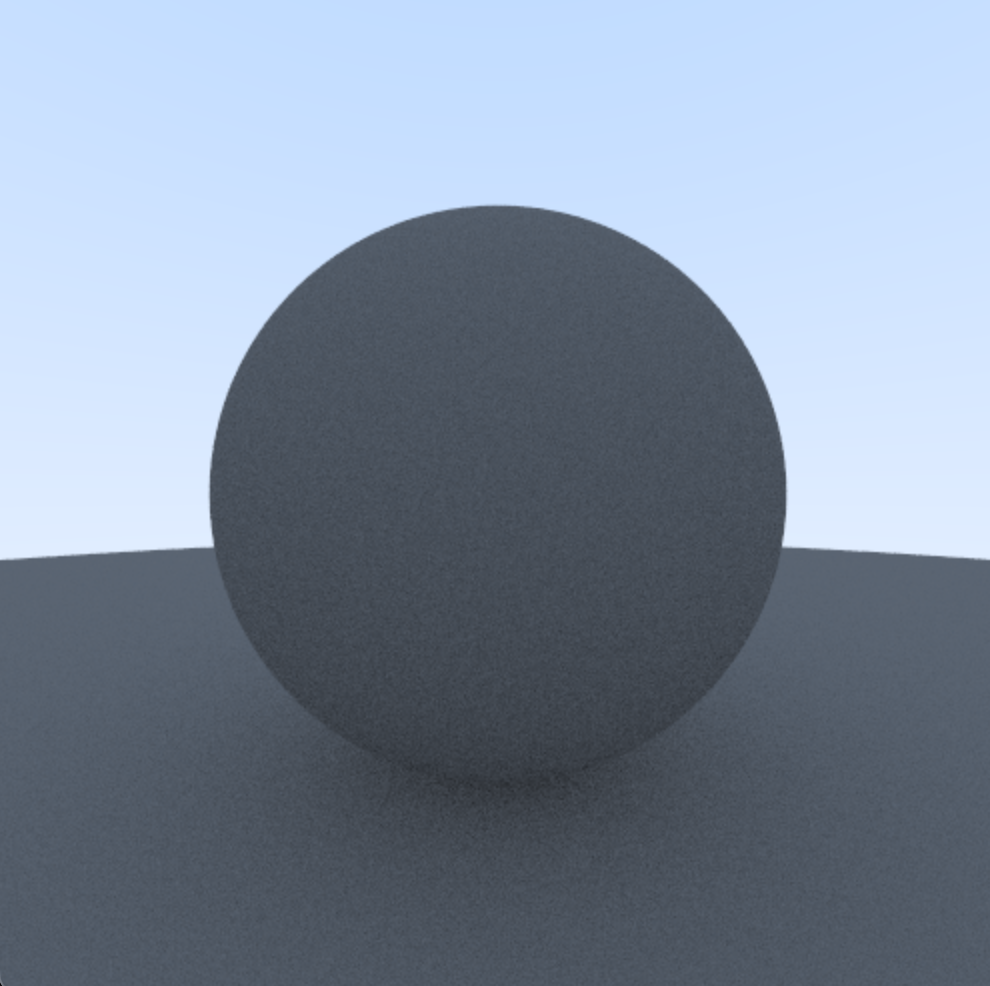
\includegraphics[width=\textwidth]{images/uniform_diffuse.png}
        \caption{Rendered image using Uniform Diffuse Renderer}
        \label{fig:completely_diffuse}
    \end{subfigure}
    \hfill
    \begin{subfigure}[b]{0.45\textwidth}
        \centering
        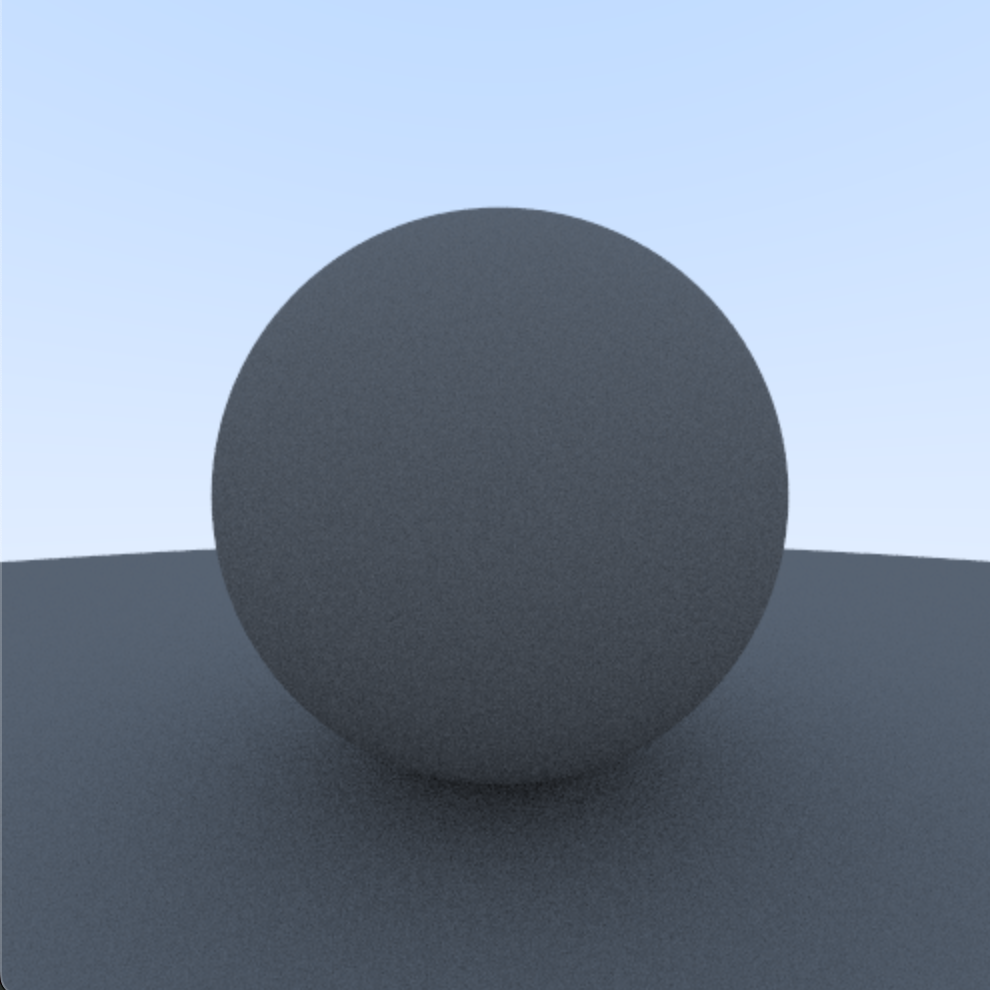
\includegraphics[width=\textwidth]{images/lambertian_diffuse.png}
        \caption{Rendered image using Lambertian Diffuse Renderer}
        \label{fig:lambertian_diffuse}
    \end{subfigure}
    \caption{Comparison of rendering techniques}
    \label{fig:rendering_comparison}
\end{figure}

*Specular Reflectance:* For specular materials, the direction of the reflected ray is computed using the reflection equation. This is crucial for simulating shiny surfaces such as metals and mirrors.

\section{Camera Dynamics}
\label{sec:camera}

\subsection{Camera and Viewing}
\label{subsec:camera-viewing}

\subsubsection{Camera Model and Rays}
The camera in ray tracing simulates the viewpoint from which the scene is rendered. It projects rays from its origin through each pixel on the image plane, capturing the scene from a specific perspective. The mathematical foundation underlying the camera's functionality involves various concepts from linear algebra.

\paragraph{Basis Vectors and Camera Orientation}

\subparagraph{Basis Vectors}
The camera's orientation is defined by three orthonormal basis vectors: \(\mathbf{u}\), \(\mathbf{v}\), and \(\mathbf{w}\).
\begin{itemize}
    \item \(\mathbf{w}\): Vector pointing from the camera position to the view direction. It is computed as:
          \[
              \mathbf{w} = \frac{\mathbf{C} - \mathbf{L}}{\|\mathbf{C} - \mathbf{L}\|}
          \]
          where \(\mathbf{C}\) is the camera position and \(\mathbf{L}\) is the focal point.
    \item \(\mathbf{u}\): Vector pointing to the right of the camera, computed using the cross product of the up vector \(\mathbf{v}_{\text{up}}\) and \(\mathbf{w}\):
          \[
              \mathbf{u} = \frac{\mathbf{v}_{\text{up}} \times \mathbf{w}}{\|\mathbf{v}_{\text{up}} \times \mathbf{w}\|}
          \]
    \item \(\mathbf{v}\): Vector pointing upwards relative to the camera, computed as:
          \[
              \mathbf{v} = \mathbf{w} \times \mathbf{u}
          \]
\end{itemize}

These basis vectors form a right-handed coordinate system and define the camera's orientation.

\paragraph{Viewport and Field of View}
The camera's field of view (FOV) determines the extent of the observable world. The vertical FOV (\(\text{vertFov}\)) is the angle of the observable world in the vertical direction:
\[
    \text{viewportHeight} = 2 \cdot \tan\left(\frac{\text{vertFov}}{2}\right)
\]
The viewport width is adjusted according to the aspect ratio (\(\text{aspectRatio}\)):
\[
    \text{viewportWidth} = \text{aspectRatio} \cdot \text{viewportHeight}
\]

\paragraph{Perspective Projection}
To generate rays from the camera through each pixel, we calculate the position of each pixel in the camera's coordinate system. The pixel positions are offset from a reference point (the upper-left corner of the viewport) by the basis vectors \(\mathbf{u}\) and \(\mathbf{v}\).

\subsubsection{Technical Implementation}

\paragraph{Initialization and Basis Vector Calculation}
The `initialize` method sets up the camera's coordinate system using the basis vectors:

\begin{verbatim}
void Camera::initialize() {
    float theta = glm::radians(vert_fov);
    float h = tan(theta / 2);
    float viewport_height = 2.0f * h;
    float viewport_width = viewport_height * float(image_width) / float(image_height);

    w = glm::normalize(center - look_at);
    u = glm::normalize(glm::cross(vup, w));
    v = glm::cross(w, u);

    pixel00_loc = center - (u * viewport_width / 2.0f) - (v * viewport_height / 2.0f) - w;
    pixel_delta_u = u * viewport_width / float(image_width);
    pixel_delta_v = v * viewport_height / float(image_height);
}
\end{verbatim}

Here,
\begin{itemize}
    \item \(\mathbf{w}\) is calculated as the normalized vector from the camera position to the look-at point.
    \item \(\mathbf{u}\) is the normalized cross product of the up vector and \(\mathbf{w}\).
    \item \(\mathbf{v}\) is the cross product of \(\mathbf{w}\) and \(\mathbf{u}\).
\end{itemize}

\paragraph{Ray Generation}
The method `getRandomRay` generates rays from the camera through each pixel, considering anti-aliasing by randomly offsetting the ray within the pixel:

\begin{verbatim}
Ray Camera::getRandomRay(int x, int y) const {
    float u_offset = (x + random_float()) * recip_sqrt_sppf;
    float v_offset = (y + random_float()) * recip_sqrt_sppf;
    glm::vec3 ray_origin = center;
    glm::vec3 ray_direction = glm::normalize(pixel00_loc + u_offset * pixel_delta_u + v_offset * pixel_delta_v - center);
    return Ray(ray_origin, ray_direction);
}
\end{verbatim}

This method uses the basis vectors to compute the direction of the rays passing through each pixel, incorporating random offsets to achieve anti-aliasing. This process ensures that each pixel's color is the result of multiple samples, reducing aliasing and producing a smoother image.

\section{Acceleration Structures}
\label{sec:acceleration-structures}
\subsection{Bounding Volume Hierarchies (BVH)}
\subsubsection{Overview of BVH}
An advanced structure for efficient intersection tests.
\subsubsection{Technical Implementation}
\begin{itemize}
    \item \textbf{Efficient Ray-Object Intersection Tests:} Using BVH for faster intersection calculations.
    \item \textbf{Building and Traversing BVH:} Methods for constructing and navigating BVH structures.
\end{itemize}
\subsubsection{Algorithmic Analysis}
Performance analysis of BVH algorithms for various scene complexities.

\section{Monte Carlo Methods for Ray Tracing}
\label{sec:monte-carlo}

\subsection{Probability and Monte Carlo Methods}
\subsubsection{Improved Random Sampling}
Stochastic methods improve sampling efficiency in rendering.

\subsubsection{Monte Carlo Integration}
Using random sampling to approximate integrals in light transport.

\subsubsection{Importance Sampling}
Advanced sampling techniques enhance efficiency and image quality.

\subsection{Integration for Lighting Models}
\subsubsection{Radiance and Light Transport Equations}
Mathematical models for light behavior in rendering.

\subsubsection{Numerical Integration Techniques}
Applying numerical methods to solve lighting equations.

\subsubsection{Technical Implementation}
Implementing global illumination and integrating direct and indirect lighting.

\section{Technical Description of the System}
\label{sec:system-description}

\subsection{System Architecture}
\subsubsection{Overview of Core Components and Their Interactions}
Core components such as Scene Manager, Camera Module, and Renderer interact seamlessly to simulate realistic lighting.

\subsubsection{Main Control Loop's Role in Managing Rendering Operations}
The main control loop orchestrates rendering, coordinating ray generation, shading, and image synthesis.

\subsubsection{Design Principles Behind the Modular Architecture}
Modular design facilitates maintenance, scalability, and integration of new features.

\subsection{Core Components}
\subsubsection{Scene Manager: Object Storage and Scene Graph Management}
The Scene Manager organizes objects in a scene graph, optimizing rendering operations.

\subsubsection{Camera Module: Virtual Camera Settings and Primary Ray Generation}
Simulates camera properties and generates primary rays for rendering.

\subsubsection{Renderer: Ray Generation and Intersection Handling}
Handles ray generation and calculates light interactions with surfaces.

\subsubsection{Geometry: An Abstraction for Hittable Objects}
Provides a unified interface for diverse geometrical shapes.

\subsubsection{Bounding Structures: Use of BVH for Efficient Intersection Tests}
Employs BVH for accelerated intersection tests, enhancing performance.

\subsection{Utilising OpenGL for Visualising Convergence}
\subsubsection{Texture Mapping: Mapping the Progressively Converging Image}
Textures are mapped to 3D models using OpenGL shaders, enhancing visual detail.

\section{Conclusion}
\label{sec:conclusion}
\subsection{Summary of Key Points}
Monte Carlo methods effectively enhance path tracing and image synthesis, improving quality and efficiency.

\subsection{Future Work}
Future exploration of advanced sampling strategies and optimizations for real-time rendering.

\subsection{Final Thoughts}
Statistical methods are crucial for high-quality rendering solutions.

\section{References}
\label{sec:references}
\bibliographystyle{plain}
\bibliography{references}


\appendix
\section{Detailed Mathematical Derivations}
\label{sec:appendix-derivations}

\section{Code Snippets and Pseudocode}
\label{sec:appendix-code}

\section{Additional Figures and Diagrams}
\label{sec:appendix-figures}

\end{document}
